\section{DST}
 From the plot of the determinant squared of $S$ as a function of $n$ for $n$
 from 1 to 32 shown in Figure~\ref{fig:S(n)}, it can be seen that the
 determinant has strictly discrete values of either 1 or -1, and follows a
 sinusoidal pattern. It is also noticeable that the plot is an odd function.

 \begin{figure}[h!]
   \centering
   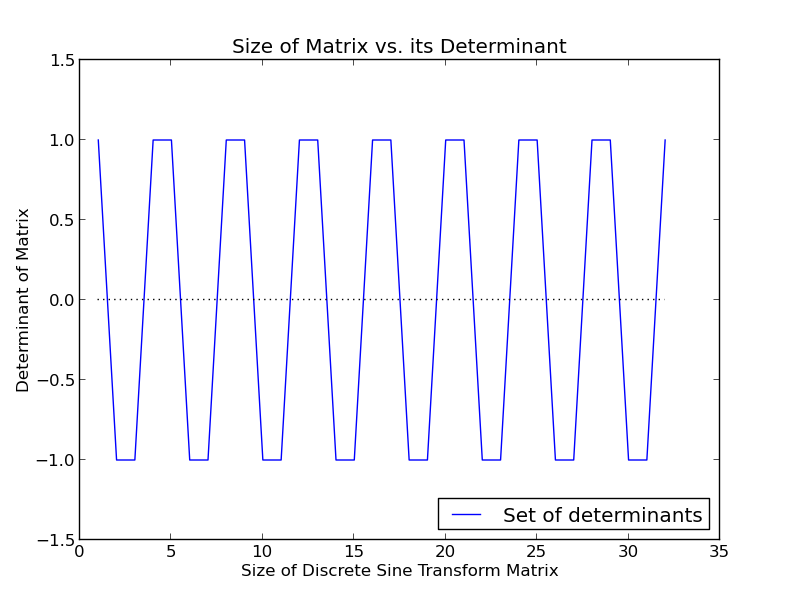
\includegraphics[scale=0.6]{./img/dst_dets.png}
   \caption{$\Delta^2$ of $S(n)$}
   \label{fig:S(n)}
\end{figure}

 The Discrete Sine Transform has the following equation:
  \begin{equation}
   \label{eq:dst}
    S_{i,j}=\sqrt{\frac{2}{n}}sin \bigg(
    \frac{\pi(i-\frac{1}{2})(j-\frac{1}{2})}{n}\bigg)
   \end{equation}  
